\documentclass{article}
\usepackage{tikz}

\renewcommand{\figurename}{Fig.}

\begin{document}

\begin{figure}[ht]
\centering

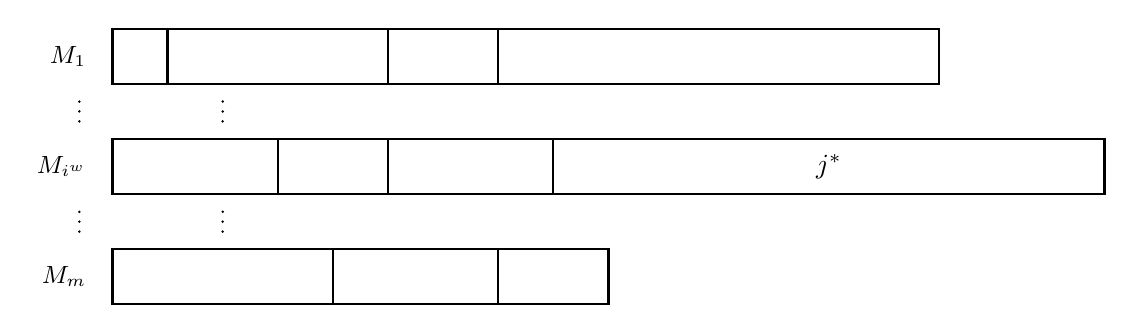
\begin{tikzpicture}[
    x=0.7cm,
    y=0.7cm,
    job/.style={
        draw,
        thick,
        fill=white,
        font=\small
    },
    machine/.style={font=\small}
]

% ------------------------------------------------
% Template idea:
% row      = displayed vertical row in the picture
% machine  = actual machine label shown on the left
%
% Use \machinerow{row}{machine label}
% Use \dotsrow{row}
% Use \jobblock{row}{start}{length}{job label}
% Use \jobblock[gray!25]{row}{start}{length}{job label} for shading
% ------------------------------------------------

\newcommand{\machinerow}[2]{
    \node[machine, anchor=east] at (-0.3,-#1+0.5) {$M_{#2}$};
}

\newcommand{\dotsrow}[1]{
    \foreach \dy in {-0.18,0,0.18} {
        \fill (-0.6,{-#1+0.5+\dy}) circle[radius=0.025];
        \fill (2,{-#1+0.5+\dy}) circle[radius=0.025];
    }
}

\newcommand{\jobblock}[5][white]{
    \draw[job, fill=#1] (#3,-#2) rectangle ++(#4,1);
    \node at ({#3 + #4/2},{-#2 + 0.5}) {$#5$};
}

% Displayed machine rows
\machinerow{1}{1}
\dotsrow{2}
\machinerow{3}{i^{w}}
\dotsrow{4}
\machinerow{5}{m}

% Example jobs
\jobblock{1}{0}{1}{}
\jobblock{1}{4}{7}{}
\jobblock{1}{1}{4}{}
\jobblock{1}{7}{8}{}

\jobblock{3}{0}{3}{}
\jobblock{3}{3}{2}{}
\jobblock{3}{5}{3}{}
\jobblock{3}{8}{10}{j^{*}}

\jobblock{5}{0}{4}{}
\jobblock{5}{4}{3}{}
\jobblock{5}{7}{2}{}

\end{tikzpicture}

\caption{$S_{WORST}(I)$}
\label{fig:schedule-structure}

\end{figure}

\end{document}